\chapter{Trace Encoder Output Packet}

Figure \ref{fig:packet-format} gives an example basic structure of the
packet energing from the encoder. This gives an example of how the
payload maybe encapsulated. Different instantiations or
implementations may have different encapsulating structures. These
would typically be dependent upon such things as the trace routing
infrastructure within the SoC.

The remainder of this section describes the contents of the Payload
portion which should be independent of the infrastructure..

\begin{figure}[h]
\begin{center}
  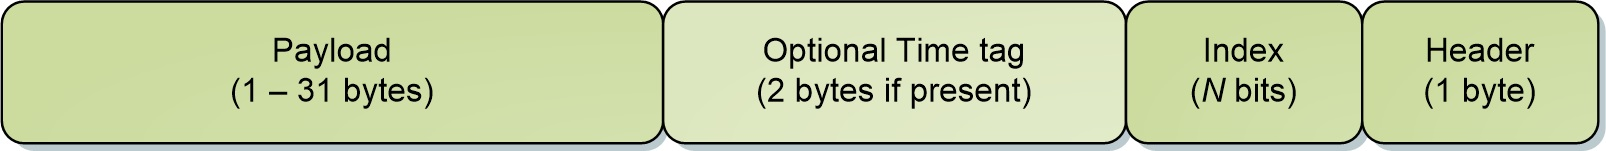
\includegraphics[height=1cm, width=9cm]{newPacket.jpg}
  \caption{Packet Format}
  \label{fig:packet-format}
\end{center}
\end{figure}


This packet payload format is used to output encoded instruction
trace.  Four different formats are used according to the needs of the
encoding algorithm. The following tables show the format of the
payload - i.e. not including the optional timestamp and not including
the the index and header.

\begin{table}[htp]
    \centering
    \caption{Packet Payload Format 0 and 1}
    \label{tab:te_inst0-1}
    \begin{tabulary}{\textwidth}{|l|p{35mm}|p{80mm}|}
        \hline
        {\bf Field name} & {\bf Bits} & {\bf Description} \\
        \hline
        \textbf{format}	& 2	& 00 (full-delta): includes branch map and full address \newline
                        01 (diff-delta): includes branch map and differential address\\
        \hline
        \textbf{branches} & 5 & Number of valid bits in branch-map. The length of branch-map is determined as follows: \newline
        0:      31 bits (\textbf{address} is not valid) \newline
        1: 	1 bit \newline
        2-9: 	9 bits \newline
        10-17: 	17 bits \newline
        18-25: 	25 bits \newline
        26-31: 	31 bits \newline
        For example if branches = 12, the branch-map is 17 bits long, and the 12 LSBs are valid. \newline
        In most cases when the branch map is full there is no need to report an address,
        and this is indicated by setting branches to 0.  The exception to this is when 
        the instruction immediately prior to the final branch causes an unpredictable discontinuity.\\
        \hline
        \textbf{branch-map} & Number of bits \newline 
                     determined by \newline 
                     \textbf {branches} field & 
                     An array of bits indicating whether branches are taken or not.\newline
        Bit 0 represents the oldest branch instruction executed.   For each bit: \newline
        0: branch taken \newline
        1: branch not taken \\
        \hline
        \textbf{address}	& Number of bits \newline 
                  is \textit {iaddress\_width\_p - iaddress\_lsb\_p} & 
                    Differential or full instruction address, according to \textbf {format}.  \newline
                    When branches is 0, the address is invalid, and is formed by sign extending branch-map.\\
        \hline
    \end{tabulary}
\end{table}


\begin{table}[!h]
    \centering
    \caption{Packet Payload Format 2}
    \label{tab:te_inst2}
    \begin{tabulary}{\textwidth}{|l|p{35mm}|p{80mm}|}
        \hline
        {\bf Field name} & {\bf Bits} & {\bf Description} \\
        \hline
        \textbf{format}	& 2	& 10 (addr-only): address and no branch map\\
        \hline
        \textbf{address} & Total number of bits 
                  for address is
                  \textit {iaddress\_width\_p - iaddress\_lsb\_p}. & 
                  Address is always differential unless the encoder has been configured to only use full-address\\ 
        \hline
    \end{tabulary}
\end{table}

\begin{table}[htp]
    \centering
    \caption{Packet Payload Format 3}
    \label{tab:te_inst3}
    \begin{tabulary}{\textwidth}{|l|p{35mm}|p{80mm}|}
      \hline
          {\bf Field name} & {\bf Bits} & {\bf Description} \\
          \hline
          \textbf{format} & 2 & 11 (sync): synchronisation\\
          \hline
          \textbf{subformat} & 2 & Sync sub-format omits fields when not required: \newline
          00 (start): ecause, interrupt and tval omitted \newline
          01 (exception): All fields present\newline
          10 (context): \textbf{address, branch, ecause, interrupt} and \textbf {tval} omitted \newline
          11 : reserved \\
          \hline
          \textbf{context} &  Total number of bits 
                     for context is  
                     \textit {context\_width\_p} 
                     unless  
                     \textit {nocontext\_p} is 1,  
                     in which case it is 0 & 
                     The instruction context \\
          \hline
          \textbf{privilege} & Number of bits is  
                      \textit {privilege\_width\_p} & 
                      The current privilege level \\
          \hline
          \textbf{branch} & 1 & If the address points to a branch instruction, set to 1 if the branch was not taken. 
          Has no meaning if this instruction is not a branch. \\
          \hline
          \textbf{address} & number of bits is  
                    \textit {iaddress\_width\_p - iaddress\_lsb\_p},  
                    unless subformat is 10, & 
                    Full instruction address.  Address alignment is determined by \textit {iaddress\_lsb\_p} Address must be left shifted in order to recreate original byte address \\
          \hline
          \textbf{ecause} & Number of bits is  
                   \textit {ecause\_width\_p} if  
                   subformat is 01,  
                   or 0 otherwise  
                   (no exception). & 
                   Exception cause \\
          \hline
          \textbf{interrupt} & Number of bits is  
                      1 if subformat is 01,  
                      or 0 otherwise (no exception). & 
                      Interrupt \\
          \hline
          \textbf{tval} & Number of bits is  
                 \textit {iaddress\_width\_p}  
                 if subformat is  
                 01 and \textit {notval\_p} is 
                 0, or 0 otherwise  
                 (no exception). & 
                 Trap value \\
          \hline
    \end{tabulary}
\end{table}

\begin{table}[!h]
    \centering
    \caption{te\_support payload}
    \label{tab:te_support}
    \begin{tabulary}{\textwidth}{|l|p{8mm}|p{80mm}|}
        \hline
        \textbf {Field name} & \textbf {Bits} & \textbf {Description} \\
        \hline
        \textbf{msg\_type}	& 2	& Set to 0x0\\
        \hline
        \textbf{control\_code} & 6 & Set to 0x34 \\
        \hline
        \textbf{support\_type} & 4 & Set to 0 to indicate \textit{itrace\_status} \\
        \hline
        \textbf{enable} & 1 & Value of \textbf {trace\_enable}\\
        \hline
        \textbf{encoder\_mode} & 2 & Value of \textbf {encoder\_mode}\\
        \hline
        \textbf{qual\_status} & 2 & Indicates qualification status\newline
          00 (no\_change): No change to filter qualification \newline
          01 (ended\_rep): Qualification ended, preceding \textbf {te\_inst} sent explicitly to indicate last qualification instruction\newline
          10: Reserved\newline
          11 : (ended\_ntr): Qualification ended, no unreported instructions (so preceeding \textbf {te\_instr} would have been sent anyway, even if it wasn't the last qualified instruction)\\
        \hline
    \end{tabulary}
\end{table}
